\section{Анализ подходов к разработке интеллектуальной системы мониторинга рисков и обеспечения безопасности путешественников}
\label{sec:analysis}

В данном разделе проводится глубокий и всесторонний анализ сферы управления рисками в путешествиях, исследуются существующие на рынке аналогичные решения и выявляются их недостатки. Также подробно рассматриваются источники данных о глобальных событиях, проводится сравнительный анализ архитектурных подходов и обосновывается выбор конкретных технологий, фреймворков и моделей машинного обучения, необходимых для реализации интеллектуальной системы мониторинга и оповещения.

\subsection{Анализ предметной области}

Системы управления рисками в путешествиях представляют собой комплексные программно-аппаратные и организационные решения, предназначенные для заблаговременного выявления, оценки, мониторинга и минимизации угроз, с которыми могут столкнуться сотрудники корпораций или частные путешественники. Развитие глобализации и увеличение объемов международных перемещений привели к тому, что обеспечение безопасности поездок стало одной из ключевых задач корпоративного управления.

Современная концепция управления рисками в путешествиях базируется на принципе «должной осмотрительности», согласно которой организация несет юридическую и моральную ответственность за безопасность своих сотрудников, находящихся в командировках. В 2021 году был опубликован международный стандарт ISO 31030 «Управление рисками в путешествиях — руководство для организаций»\cite{iso_31030_bib}, который систематизировал подходы к оценке рисков и установил высокие требования к системам мониторинга. Данный стандарт подчеркивает необходимость не только реактивного реагирования на инциденты, но и проактивного анализа потенциальных угроз еще на этапе планирования поездки. Экономические последствия пренебрежения данными стандартами могут быть катастрофическими для бизнеса. Они включают в себя не только прямые финансовые потери от необходимости экстренной медицинской эвакуации, репатриации или отмены сложных маршрутов (стоимость которых может достигать сотен тысяч долларов), но и масштабные репутационные издержки, а также многомиллионные судебные иски со стороны пострадавших сотрудников. Кроме того, современные исследования в области организационной психологии показывают, что отсутствие видимой, понятной и надежной системы обеспечения безопасности критически снижает лояльность персонала и эффективность выполнения командировочных задач из-за повышенного уровня фонового стресса в незнакомой среде. В связи с этим парадигма корпоративной безопасности окончательно сместилась от пассивного страхования рисков постфактум к активному технологическому мониторингу и превентивному управлению маршрутами на основе данных объективного контроля.

Ландшафт глобальных угроз в середине 2020-х годов характеризуется высочайшей динамичностью, непредсказуемостью и каскадным эффектом, когда природные катаклизмы мгновенно провоцируют техногенные аварии и социальные волнения. В рамках исследования предметной области была разработана расширенная таксономия рисков:
\textbf{Геополитические и социально-политические риски:}
    \begin{itemize}
    \item вооруженные конфликты, локальные боестолкновения и пограничные инциденты;
    \item государственные перевороты, резкая смена политических режимов и гражданское неповиновение;
    \item массовые протесты, забастовки работников транспортной отрасли и гражданские беспорядки;
    \item террористические акты, угрозы экстремистской деятельности и диверсии на объектах инфраструктуры;
    \item дипломатические инциденты, изменения в визовой политике и введение санкционных ограничений.
    \end{itemize}
\textbf{Природные и климатические риски:}
    \begin{itemize}
    \item сейсмическая активность, включающая землетрясения различной магнитуды и угрозы возникновения цунами;
    \item метеорологические экстремумы, такие как ураганы, тайфуны, наводнения и аномальные температурные волны;
    \item лесные пожары, извержения вулканов и пылевые бури, ограничивающие видимость и работу авиации;
    \item долгосрочные климатические изменения, влияющие на устойчивость инфраструктуры конкретного региона.
    \end{itemize}
\textbf{Эпидемиологические и медицинские угрозы:}
    \begin{itemize}
    \item вспышки инфекционных заболеваний, локальные очаги эпидемий и глобальные пандемии;
    \item низкий уровень развития местной системы здравоохранения и дефицит квалифицированного персонала;
    \item отсутствие доступа к специфическим медикаментам или качественной скорой помощи;
    \item специфические санитарно-гигиенические риски, связанные с качеством воды и пищевых продуктов.
    \end{itemize}
\textbf{Криминальные и кибернетические угрозы:}
    \begin{itemize}
    \item уличная преступность, нападения с целью грабежа и мошенничество в отношении туристов;
    \item похищения людей с целью выкупа или политического давления;
    \item кибершпионаж через публичные незащищенные сети связи и фишинговые атаки;
    \item кража персональных данных, документов и физических носителей информации у путешественников.
    \end{itemize}
\textbf{Техногенные и инфраструктурные риски:}
    \begin{itemize}
    \item аварии на объектах критической инфраструктуры, включая энергетические и водопроводные сети;
    \item масштабные сбои в работе транспортных узлов, аэропортов и железнодорожных вокзалов;
    \item энергетические кризисы, приводящие к веерным отключениям электричества и связи.
    \end{itemize}

В ходе проведенного исследования установлено, что эффективность любой системы мониторинга определяется «индексом своевременности оповещения» — временным интервалом между возникновением инцидента и получением уведомления конечным пользователем. Для глобальных систем этот показатель должен стремиться к значениям менее 15 минут, что невозможно реализовать без глубокой автоматизации процессов сбора и анализа данных.
Сфера управления рисками в путешествиях трансформировалась из узкоспециализированной области безопасности в критически важный элемент корпоративного управления и личной безопасности. Современные стандарты, такие как ISO 31030\cite{iso_31030_bib}, диктуют необходимость создания систем, способных обрабатывать огромные потоки информации в режиме реального времени. Выявленная таксономия рисков демонстрирует многогранность угроз, что требует применения междисциплинарного подхода при проектировании архитектуры интеллектуальной системы.

\subsection{Анализ сценариев использования и пользовательских ожиданий}

С точки зрения конечного пользователя ценность системы определяется не только точностью выявления угроз, но и тем, насколько быстро, понятно и в подходящем канале пользователь получает информацию. Путешественник ожидает, что система будет работать как фоновый защитный контур: заранее предупреждать о рисках при планировании маршрута, отображать актуальные события на карте, позволять уточнять картину по категориям угроз и доставлять критические сообщения даже в ситуациях, когда пользователь не находится в веб-интерфейсе.

В рамках анализа выделены ключевые сценарии использования, которые должны быть отражены как в функциональной модели, так и в пользовательском интерфейсе системы:
\begin{itemize}
    \item регистрация и авторизация пользователя должны обеспечивать безопасный доступ к персональным маршрутам, настройкам уведомлений и истории взаимодействия с системой;
    \item мониторинг инцидентов и событий безопасности должен быть доступен как обычным пользователям (для оценки рисков в рамках планирования личных поездок), так и менеджерам по управлению рисками для глобального контроля обстановки и обеспечения безопасности сотрудников;
    \item просмотр карты рисков должен предоставлять пользователям и менеджерам оперативное представление о текущей обстановке в выбранном регионе с визуальным выделением зон влияния инцидентов;
    \item фильтрация событий по типу угрозы, уровню критичности и времени публикации должна помогать быстро отделять значимые риски от фонового информационного шума в зависимости от задач конкретной роли;
    \item настройка маршрута поездки должна позволять системе сопоставлять планируемые перемещения пользователя с геометрией активных зон риска и выявлять потенциальные пересечения;
    \item получение уведомлений о безопасности должно включать как мгновенные сообщения в интерфейсе, так и оповещения по электронной почте для случаев, когда приложение закрыто;
    \item получение почтовых уведомлений должно обеспечивать доставку структурированного сообщения с названием события, уровнем угрозы, кратким описанием, регионом риска и практической рекомендацией;
    \item мониторинг состояния сервисов должен давать администратору возможность контролировать работоспособность конвейера сбора, анализа, хранения и доставки уведомлений.
\end{itemize}

Отдельного внимания требует сценарий получения почтовых уведомлений, так как он является резервным и юридически значимым каналом коммуникации. В отличие от мгновенного уведомления, которое может быть ограничено настройками мобильной операционной системы, сообщение электронной почты сохраняется в почтовом ящике пользователя, может быть повторно открыто позднее и подходит для документирования факта информирования в рамках принципа должной осмотрительности. Поэтому система должна формировать письма автоматически, на языке, выбранном пользователем, с минимальным количеством лишней информации и с четкой структурой, позволяющей быстро оценить угрозу даже в стрессовой ситуации.

\subsection{Анализ подходов к решению задачи}

При разработке систем мониторинга безопасности путешественников выделяют три фундаментальных подхода к сбору и обработке данных, каждый из которых имеет свои преимущества и ограничения.

Первый подход — экспертно-аналитический. Он основан на работе штатных аналитиков, которые вручную отбирают новости из проверенных источников, проводят верификацию данных через собственные каналы и формируют аналитические отчеты.
Преимущества данного подхода:
\begin{itemize}
\item высочайшая точность, глубина контекстуального анализа и достоверность предоставляемых сведений;
    \item практически полное отсутствие ложных срабатываний, вызванных метафоричностью или иронией в текстах;
    \item возможность составления долгосрочного прогноза развития ситуации на основе инсайдерской информации.
\end{itemize}
Недостатки:
\begin{itemize}
\item критически низкая скорость реакции на динамические инциденты из-за человеческого фактора;
    \item чрезвычайно высокая стоимость содержания круглосуточного штата высококвалифицированных аналитиков;
    \item ограниченность масштабирования, не позволяющая одновременно отслеживать тысячи локальных источников на разных языках.
\end{itemize}

Второй подход — алгоритмический сбор на основе ключевых слов и регулярных выражений. Системы настраиваются на автоматический поиск определенных комбинаций слов в новостных лентах и социальных сетях.
Преимущества:
\begin{itemize}
\item высокая скорость первичной обработки данных и возможность охвата большого количества источников;
    \item относительно низкая стоимость реализации и простота технической поддержки алгоритмов.
\end{itemize}
Недостатки:
\begin{itemize}
\item критически высокий уровень информационного шума и ложных срабатываний на нерелевантные новости;
    \item значительные трудности с автоматическим определением точной геолокации и границ зоны инцидента;
    \item неспособность алгоритмов понимать сложный контекст, тональность сообщения и выявлять дезинформацию.
\end{itemize}

Третий подход — интеллектуальный анализ с применением обработки естественного языка и современных моделей машинного обучения. Данный подход предполагает использование глубоких нейронных сетей для семантического разбора текста, извлечения сущностей и автоматической многофакторной классификации.
Преимущества:
\begin{itemize}
\item практически мгновенная обработка входящего потока информации в режиме реального времени;
    \item глобальный охват источников на множестве языков без необходимости пропорционального расширения штата;
    \item возможность автоматического геокодирования и динамической оценки уровня серьезности каждого инцидента.
\end{itemize}
Недостатки:
\begin{itemize}
\item высокая инженерная сложность разработки, обучения и интеграции нейросетевых моделей;
    \item значительная требовательность к вычислительным ресурсам, особенно при использовании больших языковых моделей;
    \item необходимость внедрения механизмов постоянного дообучения моделей на свежих данных для сохранения точности.
\end{itemize}

В результате проведенного анализа подходов к решению задачи, наиболее предпочтительным к реализации признан третий подход, дополненный гибридными механизмами автоматической проверки достоверности, что позволяет эффективно объединить скорость алгоритмов с качеством экспертной аналитики. Важно отметить, что применение исключительно нейросетевых моделей сопряжено с проблемой так называемого «дрейфа концептов» (concept drift). Язык описания угроз в мировых СМИ постоянно эволюционирует: регулярно появляются новые термины для обозначения кибератак, специфические названия новых вирусных штаммов или аббревиатуры недавно сформированных локальных вооруженных группировок, на которых базовая модель физически не могла быть обучена.

Для компенсации этого эффекта гибридный подход подразумевает глубокую интеграцию классических детерминированных правил и математических эвристик поверх вероятностного нейросетевого вывода. Например, если трансформерная модель сомневается в итоговой классификации события из-за нестандартной формулировки журналиста, но в тексте с помощью регулярных выражений обнаружены жестко заданные маркеры экстремальной опасности (такие как уровень магнитуды землетрясения в баллах или радиус эвакуации в километрах), система принудительно повышает приоритет инцидента. Сравнение различных методологий обработки информации показало, что традиционные методы изолированно абсолютно не справляются с современными объемами данных и требованиями к скорости оповещения. Интеллектуальный подход на базе обработки естественного языка позволяет решить проблему масштабируемости и многоязычности, обеспечивая при этом высокий уровень точности за счет использования современных трансформерных архитектур. Таким образом, внедрение гибридных технологий машинного обучения является безальтернативным путем для создания гибкой, надежной и конкурентоспособной системы глобального мониторинга рисков.

\subsection{Анализ аналогов системы}

На мировом рынке представлено несколько крупных систем мониторинга рисков, ориентированных преимущественно на корпоративный сегмент, где заказчиками выступают крупные корпорации, страховые компании или глобальные туристические операторы. В качестве аналогов были проанализированы следующие системы: International SOS, Safeture, Crisis24.

\textbf{International SOS} является признанным мировым лидером в области медицинского сопровождения и обеспечения безопасности. Их система мониторинга опирается на уникальную сеть из 27 центров помощи и тысячи штатных экспертов. На рисунке \ref{fig:isos} представлен пользовательский интерфейс мобильного приложения системы.

\begin{figure}[h]
\centering
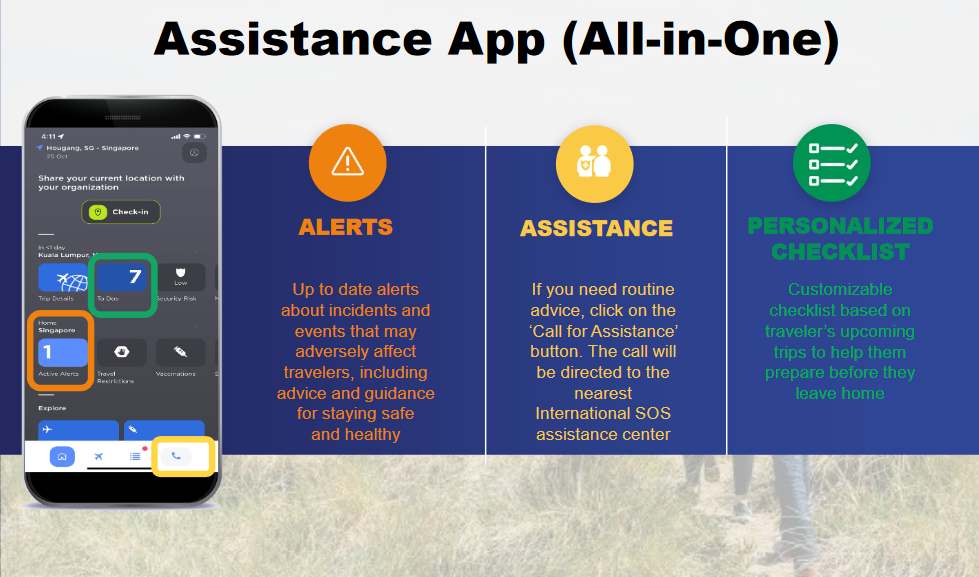
\includegraphics[width=1\textwidth]{picture/international-sos.png}
\caption{Пользовательский интерфейс мобильного приложения International SOS}
\label{fig:isos}
\end{figure}

Особенности системы:
\begin{itemize}
\item бесшовная интеграция с корпоративными системами бронирования билетов и отелей через модуль TravelTracker;
\item наличие выделенной кнопки экстренной связи для мгновенного соединения с оператором ситуационного центра;
\item наличие глубокой и проверенной экспертизы в области экстренной медицины и организации эвакуации.
\end{itemize}

Главным недостатком системы International SOS является ее закрытая экосистема и крайне высокая стоимость подписки, что делает решение недоступным для малого бизнеса и самостоятельных туристов. Также наблюдается определенная задержка в обновлении оперативных данных о быстроразвивающихся инцидентах из-за обязательного этапа ручной верификации каждой новости аналитиком.

\textbf{Safeture} представляет собой современную технологическую платформу из Швеции, сфокусированную на инструментах отслеживания местоположения и управления мобильностью персонала в реальном времени. Пользовательский интерфейс платформы Safeture показан на рисунке \ref{fig:safeture}.

\begin{figure}[h]
\centering

\includegraphics[width=1.0\textwidth]{picture/safeture.png}
\caption{Пользовательский интерфейс платформы Safeture}
\label{fig:safeture}
\end{figure}

Особенности системы:
\begin{itemize}
\item мощный встроенный модуль геопозиционирования с функциями интеллектуального геофенсинга и контроля зон;
\item автоматическая рассылка уведомлений пользователям на основе их точного географического местоположения;
\item наличие надежных инструментов для организации двухсторонней связи между сотрудником и службой безопасности.
\end{itemize}

Критическим ограничением платформы Safeture является ее зависимость от внешних поставщиков разведывательных данных, так как компания не проводит собственного первичного анализа новостных потоков. Система функционирует как высокотехнологичный агрегатор и средство доставки информации, что ограничивает возможности контроля качества аналитики на нижнем уровне.

\textbf{Crisis24}, являясь подразделением компании GardaWorld, предлагает комплексную платформу Horizon, которая объединяет возможности искусственного интеллекта и глубокую экспертизу человеческой аналитики. Интерфейс системы Crisis24 представлен на рисунке \ref{fig:crisis24}.

\begin{figure}[h]
\centering
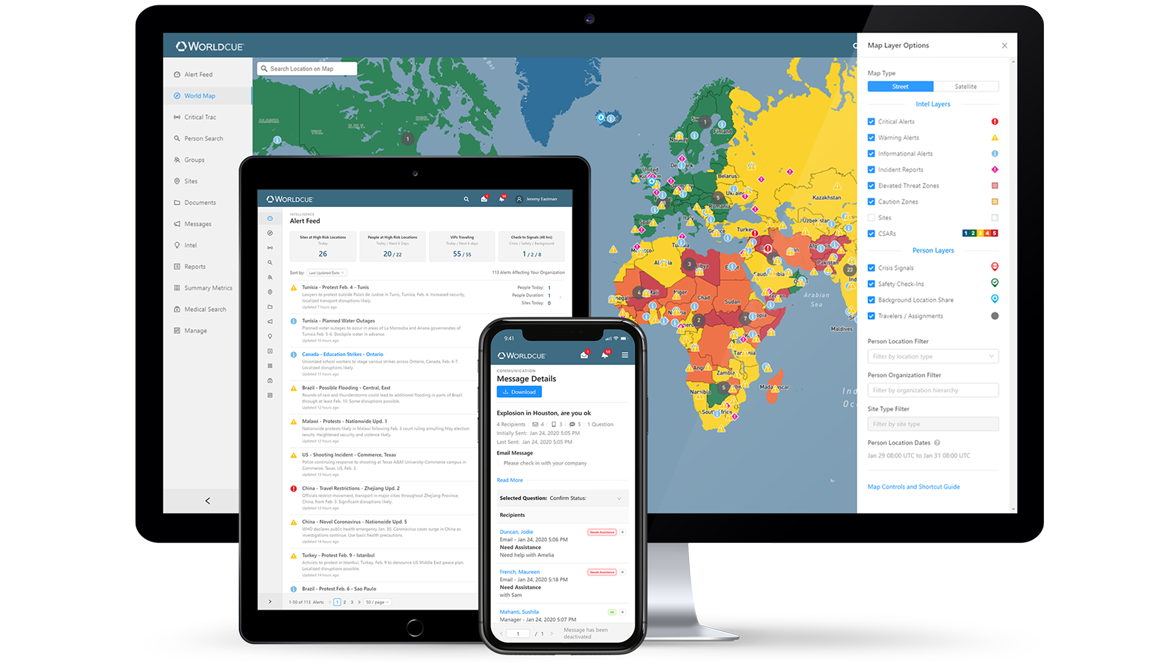
\includegraphics[width=1.0\textwidth]{picture/crisis.png}
\caption{Интерфейс системы Crisis24}
\label{fig:crisis24}
\end{figure}

Особенности системы:
\begin{itemize}
\item активное использование алгоритмов машинного обучения для первичной фильтрации и кластеризации новостей;
\item наличие обширной базы детальных страновых отчетов, охватывающей более 200 направлений по всему миру;
\item высокая гибкость настройки пороговых значений уровней риска под специфические нужды конкретной организации.
\end{itemize}

Несмотря на высокую технологичность, система Horizon остается инструментом, ориентированным на профессиональных риск-менеджеров. Ее пользовательский интерфейс зачастую перегружен сложными графиками и избыточной информацией, что может затруднить быстрое восприятие ситуации обычным путешественником в условиях стресса или дефицита времени. Разрабатываемая система призвана устранить этот барьер, предлагая интуитивно понятный интерфейс, адаптированный под задачи рядовых пользователей.

Сравнительный анализ систем мониторинга рисков в путешествиях представлен в таблице \ref{tab:analogs_comparison}, в которой отражены ключевые характеристики существующих систем.

\begin{table}[h!]
\centering
\caption{Сравнительный анализ систем мониторинга рисков в путешествиях}
\label{tab:analogs_comparison}
\begin{tabularx}{\textwidth}{|Y|C|C|C|}
\hline
\textbf{Критерий сравнения} & \textbf{Int. SOS} & \textbf{Safeture} & \textbf{Crisis24} \\ \hline
Основной источник данных & Эксперты & Агрегаторы & Гибридный \\ \hline
Скорость и метод анализа данных & Медленный (ручной труд) & Отсутствует (только сбор) & Средний (частично ручной) \\ \hline
Скорость оповещения & Средняя & Высокая & Высокая \\ \hline
Поддержка индивидуальных путешественников (B2C) & Нет & Нет & Ограничена \\ \hline
Наличие NLP-конвейера (глубокий анализ текста) & Нет (ручной анализ) & Нет & Частично \\ \hline
Автоматическое геокодирование & Нет & Да & Да \\ \hline
Интеграция с картами & Да & Да & Да \\ \hline
Локализация данных и интерфейса & Частичная & Частичная & Частичная \\ \hline
Стоимость решения & Очень высокая & Высокая & Высокая \\ \hline
\end{tabularx}
\end{table}

Проведенный детальный анализ существующих решений показывает, что на мировом рынке сохраняется свободная ниша для системы, которая способна сочетать в себе сверхвысокую скорость полностью автоматизированного анализа данных из открытых источников и доступность для широкого круга индивидуальных пользователей. 
Как видно из таблицы \ref{tab:analogs_comparison}, изучение коммерческих аналогов позволило выявить общую тенденцию к высокой стоимости и жесткой ориентации на корпоративный сектор. Эти системы не поддерживают услуги для индивидуальных путешественников, оставляя сегмент частных лиц незащищенным. Кроме того, большинство платформ либо полагаются на медленный ручной труд аналитиков (что снижает скорость анализа данных), либо выступают посредниками-агрегаторами без глубокого анализа. Разрабатываемый проект призван устранить эти недостатки за счет внедрения собственного аналитического конвейера на базе обработки естественного языка (NLP). Это обеспечит независимость от внешних провайдеров, гарантирует сверхвысокую скорость обработки данных и снизит эксплуатационные расходы.

\subsection{Анализ источников данных}

Для обеспечения полноценного глобального покрытия система должна агрегировать и обрабатывать информацию из множества гетерогенных и распределенных источников. Были проанализированы следующие ключевые категории:

\begin{itemize}
\item \textbf{проект GDELT (Global Database of Events, Language, and Tone)}\cite{gdelt_bib} --- крупнейший в мире открытый массив данных о событиях, обновляемый каждые 15 минут и содержащий ссылки на новости на 65 языках;
\item \textbf{социальные медиа и мессенджеры (Twitter, Telegram)} --- источники наиболее оперативной, но при этом характеризующейся экстремально высоким уровнем шума и дезинформации информации;
\item официальные правительственные отчеты и бюллетени (Министерства иностранных дел, МЧС): обладают высочайшей степенью достоверности, но зачастую публикуются с критической задержкой;
\item \textbf{специализированные метеорологические и сейсмические службы (GDACS, USGS)} --- источники, предоставляющие четко структурированные данные о природных катаклизмах в машиночитаемых форматах XML и JSON.
\end{itemize}

В рамках данной работы научно обосновано использование GDELT как основного информационного фундамента системы, так как этот проект обеспечивает беспрецедентную широту охвата и глубину метаданных, необходимых для дообучения нейронных сетей. Выбор GDELT в качестве базового источника обусловлен его уникальной способностью в режиме реального времени консолидировать мировые новости из десятков тысяч локальных изданий с автоматическим переводом на английский язык, что радикально упрощает разработку унифицированных моделей обработки естественного языка. Особую аналитическую ценность представляет встроенная в GDELT система кодирования событий CAMEO (Conflict and Mediation Event Observations), которая автоматически присваивает новостным сюжетам строгие числовые коды взаимодействий между акторами, а также использование шкалы Гольдштейна (Goldstein Scale) для базовой математической оценки потенциального влияния события на политическую стабильность конкретного региона.

Однако промышленная работа с массивами GDELT сопряжена с рядом серьезных инженерных вызовов. Наличие колоссального объема информационного шума, дублирующихся сообщений об одном и том же инциденте от разных информационных агентств и исторических смещений в данных требует разработки сложного многоэтапного конвейера дедупликации. Зачастую исторические ретроспективы или объемные аналитические статьи могут ошибочно маркироваться базовыми алгоритмами как текущие инциденты. Для компенсации этих недостатков требуется внедрение дополнительных эвристических фильтров по временным меткам извлекаемых сущностей.

В свою очередь, прямая обработка неструктурированных социальных медиа и профильных мессенджеров требует решения сложнейших проблем, связанных со строгими ограничениями программных интерфейсов (API Rate Limits), постоянной борьбой с бот-трафиком и целенаправленными информационными вбросами (дезинформацией). Поэтому интеграция подобных источников целесообразна только при наличии мощного программного модуля оценки достоверности (Trust Scoring) на базе графового анализа надежности источников. Интеграция же данных из строго структурированных специализированных сейсмических и метеорологических служб (например, USGS, EMSC) позволит дополнить систему точными сведениями о природных угрозах, создавая надежную многослойную информационную модель окружающего мира, где вероятностные текстовые данные органично накладываются на детерминированные физические измерения.

\subsection{Анализ требований к локализации данных и интерфейса}

Глобальный характер системы мониторинга рисков делает локализацию не вспомогательной функцией пользовательского интерфейса, а одним из базовых требований к качеству информирования. Одно и то же событие может быть обнаружено в статье BBC на английском языке, в сообщении местного издания на испанском, в официальном бюллетене на арабском или в региональном источнике на русском языке, при этом пользователь должен получить понятное описание угрозы на выбранном языке без необходимости самостоятельно интерпретировать оригинальный текст. В контексте безопасности путешественников языковой барьер напрямую влияет на скорость принятия решений, так как неточный или запоздалый перевод может привести к неправильной оценке зоны риска, уровня опасности и рекомендуемого поведения.

Локализация системы должна охватывать два уровня. Первый уровень связан с локализацией интерфейса, то есть переводом меню, фильтров, категорий угроз, статусов маршрута, подписей на карте и шаблонов уведомлений. Второй уровень связан с локализацией данных, то есть автоматическим определением языка исходного материала, сохранением исходной версии события и генерацией переводов названий, описаний и кратких рекомендаций для поддерживаемых языков. Такой подход позволяет одновременно сохранять трассируемость к оригинальному источнику и предоставлять пользователю адаптированное содержание.

\textbf{Определение языка источника информации.} На первом этапе обработки необходимо установить язык текста, из которого было извлечено событие. Для этого могут применяться алгоритмы N-граммной категоризации текста, основанные на сравнении частотных профилей символов или словоформ с заранее подготовленными профилями языков. Данный подход хорошо подходит для коротких новостных фрагментов, не требует больших вычислительных ресурсов и может быть реализован с помощью библиотек семейства Compact Language Detector, Lingua или аналогичных решений\cite{lingua_language_detector_bib}. Его преимуществом является высокая скорость и предсказуемость, однако качество снижается для смешанных текстов, заголовков с большим количеством имен собственных, транслитерации и сообщений, в которых исходный язык частично заменен цитатами.

Альтернативой являются методы машинного обучения для определения языка, включая fastText lid.176, модели на основе символьных сверточных нейронных сетей и компактные трансформерные классификаторы\cite{fasttext_language_identification_bib}. FastText представляет особый интерес для данной системы, так как он распространяется как самодостаточная модель, поддерживает большое количество языков, быстро работает на центральном процессоре и может быть развернут внутри инфраструктурного контура без обращения к внешним программным интерфейсам. Более тяжелые трансформерные модели потенциально точнее на сложных случаях, но требуют больших ресурсов и хуже подходят для высокочастотного потока GDELT, где определение языка должно выполняться до основных этапов анализа.

Облачные решения, такие как Google Cloud Translation Language Detection, AWS Comprehend или Azure AI Language, обладают высоким качеством и простым программным интерфейсом, но создают зависимость от внешнего провайдера, увеличивают операционные затраты и требуют передачи фрагментов новостных материалов за пределы системы. Для дипломного проекта это является существенным ограничением, поскольку в системе могут обрабатываться маршруты, предпочтения пользователей и корреляции между событиями и зонами присутствия путешественников. Даже если сами новости являются открытыми, связанный с ними контекст обработки может иметь конфиденциальный характер.

Сравнение подходов к определению языка источника представлено в таблице \ref{tab:language_detection_models}, в которой сопоставлены наиболее значимые показатели: точность или F1-мера на задаче определения языка, количество поддерживаемых языков, вычислительная стоимость и возможность локального развертывания.

\begin{table}[h!]
\centering
\small
\caption{Сравнение подходов к определению языка источника}
\label{tab:language_detection_models}
\begin{tabularx}{\textwidth}{|L{2.6cm}|Y|Y|Y|Y|}
\hline
\textbf{Подход} & \textbf{Основные метрики} & \textbf{Поддержка языков} & \textbf{Развертывание} & \textbf{Оценка для проекта} \\ \hline
N-граммные профили & точность, макро-F1, задержка & высокая для популярных языков & полностью локальное & быстрый базовый вариант, чувствительный к коротким смешанным текстам \\ \hline
Lingua & точность на коротких текстах, задержка & более 70 языков & полностью локальное & подходит для заголовков и коротких фрагментов без сетевых вызовов \\ \hline
fastText lid.176 & точность, макро-F1, пропускная способность & 176 языков & полностью локальное & предпочтительный вариант для потока GDELT из-за скорости и широты покрытия \\ \hline
Облачные про\-граммные интерфейсы & оценка качества провайдера, задержка, соглашение об уровне обслуживания & зависит от провайдера & внешний про\-граммный интерфейс & высокий комфорт интеграции, но есть риск раскрытия контекста обработки \\ \hline
\end{tabularx}
\end{table}

\textbf{Автоматический перевод событий, описаний и заголовков.} Задача автоматического перевода в системе отличается от обычного машинного перевода тем, что объектом обработки являются не только полные статьи, но и сжатые аналитические представления: заголовки событий, короткие описания, темы электронных писем, рекомендации и подписи на карте. Для таких данных критичны терминологическая устойчивость, сохранение географических названий, корректная передача уровня угрозы и отсутствие художественного перефразирования. Ошибка в переводе слов «предупреждение», «эвакуация», «комендантский час» или «забастовка» может существенно изменить восприятие риска.

Подход с локальным развертыванием предполагает размещение моделей перевода в собственной инфраструктуре. Для этой задачи могут применяться NLLB-200, M2M100, MarianMT и OPUS-MT, а также локальные большие языковые модели вроде Qwen2.5 или Mistral для постобработки и нормализации стиля\cite{nllb_bib,m2m100_bib,marian_nmt_bib,opus_mt_bib,qwen25_bib,mistral7b_bib}. NLLB-200 является предпочтительным базовым вариантом для многоязычной системы, так как изначально ориентирован на широкий набор языков и хорошо подходит для перевода между парами, в которых английский не всегда является единственным промежуточным языком. MarianMT и OPUS-MT рационально использовать для отдельных высоконагруженных языковых пар, например английский-русский или английский-испанский, когда требуется высокая скорость и предсказуемая стоимость инференса.

Облачные переводчики, такие как Google Cloud Translation, DeepL, Microsoft Translator и Amazon Translate, обеспечивают высокое качество на популярных языковых парах, быстро подключаются и снимают с команды часть инфраструктурной нагрузки. Их недостатки проявляются в долгосрочной эксплуатации: стоимость растет пропорционально объему переводимых текстов, доступность зависит от внешнего соглашения об уровне обслуживания, а политика обработки данных ограничивает контроль над тем, где и как сохраняются фрагменты исходных материалов. Для системы безопасности путешественников это особенно важно, так как перевод может выполняться для событий, связанных с конкретными маршрутами и настройками уведомлений пользователя.

Сравнение подходов к машинному переводу текстов событий представлено в таблице \ref{tab:translation_models}. Для машинного перевода наиболее часто используются метрики BLEU, chrF и COMET, а для промышленного внедрения дополнительно важны задержка инференса, стоимость обработки и контролируемость хранения данных.

\begin{table}[h!]
\centering
\small
\caption{Сравнение подходов к машинному переводу текстов событий}
\label{tab:translation_models}
\begin{tabularx}{\textwidth}{|L{2.6cm}|Y|Y|Y|Y|}
\hline
\textbf{Модель или сервис} & \textbf{Основные метрики} & \textbf{Языковое покрытие} & \textbf{Развертывание} & \textbf{Оценка для проекта} \\ \hline
NLLB-200 & BLEU, chrF++, COMET & около 200 языков & локальное & базовая модель для универсального перевода и редких языковых направлений \\ \hline
M2M100 & BLEU, chrF & 100 языков & локальное & полезна как альтернатива для прямого многоязычного перевода без английского посредника \\ \hline
MarianMT и OPUS-MT & BLEU, задержка, пропускная способность & зависит от языковой пары & локальное & рациональны для частых пар, где важна скорость и малый размер модели \\ \hline
Облачные переводчики & BLEU, COMET, соглашение об уровне обслуживания, стоимость за символ & широкое покрытие & внешний про\-граммный интерфейс & удобны для прототипирования, но нежелательны при обработке чувствительного контекста \\ \hline
\end{tabularx}
\end{table}

\textbf{Реферирование текстов из источников.} Помимо перевода, система должна решать задачу реферирования исходных материалов, так как пользователю в условиях поездки невозможно читать полную новостную статью, официальный бюллетень или длинный аналитический текст. Реферирование в данном контексте отличается от обычного сокращения текста: итоговая сводка должна сохранить тип угрозы, место, временной контекст, потенциальное влияние на путешественника и практический смысл события. Если модель удалит из сводки упоминание конкретного города, района аэропорта, даты начала комендантского часа или направления эвакуации, то уведомление станет формально кратким, но практически бесполезным.

Существуют два основных подхода к автоматическому реферированию. Экстрактивное реферирование выбирает из исходного текста наиболее значимые предложения без их переформулирования. Классические методы TextRank, LexRank и LSA просты, устойчивы и хорошо объяснимы, однако они плохо адаптируют стиль текста под уведомление и часто сохраняют лишние журналистские обороты, цитаты или политический контекст, не имеющий прямого отношения к безопасности путешественника\cite{textrank_bib,lexrank_bib,lsa_summarization_bib}. Более современные экстрактивные модели на основе BERT и Sentence-BERT лучше оценивают семантическую значимость предложений, но все равно ограничены тем, что не создают нового компактного описания события.

Абстрактивное реферирование генерирует новую краткую формулировку, опираясь на смысл исходного текста. Для этой задачи применяются модели BART, PEGASUS, T5, mT5, mBART, LongT5, а также современные инструкциионные большие языковые модели, такие как Qwen2.5, Mistral, Llama и их специализированные варианты\cite{bart_bib,pegasus_bib,t5_bib,mt5_bib,mbart_bib,longt5_bib,qwen25_bib,mistral7b_bib}. Преимущество абстрактивного подхода заключается в возможности привести разнородный новостной текст к единому формату: одно-два предложения для карточки события, отдельная краткая рекомендация для почтового уведомления и сжатое описание для мобильного уведомления. Недостатком является риск галлюцинаций, потери числовых деталей и искажения причинно-следственных связей, поэтому для системы безопасности требуется строгий промпт, ограниченный контекст и последующая проверка ключевых сущностей.

Отдельную сложность создает многоязычность входного потока. Формально существуют мультиязычные модели реферирования, например mT5, mBART-50 и некоторые варианты NLLB-совместимых конвейеров, однако их качество существенно различается по языкам. Для английского, русского, испанского, французского и немецкого языков можно добиться приемлемого результата, но для редких региональных языков, смешанных новостных сообщений или автоматических переводов локальных изданий качество реферирования становится менее предсказуемым. В системе мониторинга рисков это недопустимо, так как редкие языки часто встречаются именно в локальных источниках, которые первыми сообщают о региональных инцидентах.

Поэтому рациональным является двухэтапный подход: сначала определить язык источника, затем при необходимости выполнить машинный перевод на один из опорных языков, для которого реферирующая модель показывает стабильное качество, и только после этого сформировать сводку. Такой порядок увеличивает вычислительные затраты, но делает поведение системы более управляемым. Перевод может выполняться через локально развернутые NLLB-200 или MarianMT, после чего локальная большая языковая модель Qwen2.5 или Mistral генерирует краткую сводку в заданном формате. Для языков, которые модель реферирования поддерживает напрямую, перевод можно пропускать, но этот список должен быть ограничен и подтвержден тестированием на реальных новостных материалах.

Облачные модели реферирования, включая облачные большие языковые модели и специализированные программные интерфейсы анализа текста, обладают высокой гибкостью и позволяют быстро получить качественные сводки без самостоятельного обслуживания графической инфраструктуры. Однако они требуют передачи полного текста статьи и контекста события внешнему провайдеру, а иногда и дополнительных метаданных, связанных с географией угрозы или пользовательскими настройками. В рамках системы обеспечения безопасности путешественников такая зависимость создает риск раскрытия операционного контекста, усложняет соблюдение требований конфиденциальности и делает стоимость обработки трудно прогнозируемой при резком росте потока событий.

Сравнение подходов к реферированию текстов представлено в таблице \ref{tab:summarization_models}. Для данной задачи наиболее распространены метрики ROUGE-1, ROUGE-2, ROUGE-L и BERTScore, однако в системе безопасности дополнительно необходимо учитывать фактическую согласованность, сохранение именованных сущностей, длину контекста и возможность локального развертывания.

\begin{table}[h!]
\centering
\small
\caption{Сравнение подходов к реферированию текстов}
\label{tab:summarization_models}
\begin{tabularx}{\textwidth}{|L{3.2cm}|Y|Y|Y|Y|}
\hline
\textbf{Подход или модель} & \textbf{Основные метрики} & \textbf{Языковая устойчивость} & \textbf{Развертывание} & \textbf{Оценка для проекта} \\ \hline
TextRank, LexRank, LSA & ROUGE, задержка, объяснимость & зависит от токенизации & локальное & пригодны как резервный вариант, но плохо формируют текст уведомления \\ \hline
BART, PEGASUS, T5 & ROUGE, BERTScore, фактическая согласованность & в основном английский & локальное & качественны для опорного языка, но ограничены мультиязычностью \\ \hline
mT5, mBART, LongT5 & ROUGE, BERTScore, длина контекста & многоязычная, но неоднородная & локальное & полезны для экспериментов, однако требуют проверки по каждому языку \\ \hline
Qwen2.5 и Mistral & ROUGE, фактическая точность, сохранение сущностей, задержка & зависит от языка и промпта & локальное через собственную среду & предпочтительны для управляемой сводки после перевода на опорный язык \\ \hline
Облачные большие языковые модели & ROUGE, экспертная оценка, соглашение об уровне обслуживания, стоимость & широкая & внешний про\-граммный интерфейс & качественны, но конфликтуют с требованием конфиденциальности \\ \hline
\end{tabularx}
\end{table}

По результатам анализа таблиц \ref{tab:language_detection_models}, \ref{tab:translation_models} и \ref{tab:summarization_models} для проекта целесообразно выбрать гибридный стек с локальным развертыванием: fastText lid.176 или Lingua для первичного определения языка, облегченную версию NLLB-200 для универсального машинного перевода, MarianMT или OPUS-MT для наиболее частых языковых пар и локальную большую языковую модель Qwen2.5 или Mistral для реферирования и краткой стилистической нормализации уведомлений. Такой выбор обеспечивает конфиденциальность данных, снижает зависимость от коммерческих программных интерфейсов и позволяет сохранять полный контроль над журналированием, версионированием моделей и повторной обработкой событий при изменении требований к качеству локализации.

\subsection{Анализ архитектурных подходов}

При проектировании глобальной системы мониторинга критически важно обеспечить высокую масштабируемость и отказоустойчивость. Проведен сравнительный анализ трех основных архитектурных паттернов.

Традиционная монолитная архитектура была аргументированно отвергнута из-за невозможности независимого масштабирования ресурсоемких модулей машинного обучения и низкой гибкости при внесении изменений в отдельные компоненты системы.

Микросервисная архитектура с синхронным взаимодействием через REST-интерфейсы также признана неоптимальной для данной задачи. Время обработки одного новостного текста нейронными сетями может значительно варьироваться, что при синхронных вызовах неизбежно приведет к возникновению каскадных блокировок и деградации производительности.

Выбранный итоговый подход — событийно-ориентированная микросервисная архитектура (Event-Driven Architecture) с применением промышленного брокера сообщений. Данный подход позволяет эффективно решать следующие базовые задачи:
\begin{itemize}
\item полная техническая и логическая изоляция процессов непрерывного сбора, ресурсоемкого интеллектуального анализа и массовой асинхронной рассылки уведомлений пользователям;
\item гарантированная доставка (at-least-once delivery) и обработка всех накопленных данных даже при возникновении длительных временных сбоев или перезапусков в работе отдельных аналитических сервисов;
\item возможность беспрепятственного горячего внедрения новых аналитических, геоинформационных и прогностических модулей в существующий конвейер без остановки обработки основного потока.
\end{itemize}

Для успешной реализации такой архитектуры в контексте высоконагруженной системы мониторинга необходимо строгое следование ряду специфических паттернов проектирования. В первую очередь, это паттерн обеспечения идемпотентности обработки сообщений. Поскольку в распределенных системах возможна доставка одного и того же события несколько раз из-за сетевых задержек, микросервисы анализа и оповещения должны уметь распознавать дубликаты инцидентов по уникальным идентификаторам и вычисляемым хэш-суммам контента, чтобы не перегружать конечного пользователя повторяющимися уведомлениями об одной и той же угрозе. Во-вторых, критически важно применение механизмов контроля обратного давления (Backpressure), которые на уровне брокера сообщений защищают реляционную базу данных и потребителей от переполнения оперативной памяти.

\textbf{Оценка эффективности выбранной архитектурной модели.} Событийно-ориентированный подход объективно является наиболее адаптивным и отказоустойчивым для систем, работающих с крайне непредсказуемыми объемами входящих данных. Использование надежных очередей сообщений позволяет сглаживать пиковые нагрузки, неизбежно возникающие в моменты крупных мировых катаклизмов (масштабные стихийные бедствия, государственные перевороты, крупные террористические акты), когда количество публикуемых в мире профильных новостей возрастает на несколько порядков буквально за считанные минуты. В традиционной монолитной системе с синхронным взаимодействием подобный информационный всплеск неминуемо привел бы к быстрому исчерпанию пула потоков соединения с базой данных и полному отказу в обслуживании всех активных пользователей (DDoS-эффект). Выбранная же микросервисная архитектура обеспечивает высочайшую живучесть платформы: избыточные сообщения безопасно буферизуются в очередях на диске, а оркестратор контейнеров автоматически масштабирует только те компоненты, которые испытывают наибольшую нагрузку (например, инстансы с графическими ускорителями для инференса больших языковых моделей), никак не затрагивая при этом стабильность работы клиентского картографического интерфейса или критически важного модуля авторизации пользователей.
\subsection{Выбор моделей машинного обучения}

Для реализации качественного интеллектуального анализа неструктурированного текста детально рассмотрены и выбраны следующие технологические решения:
\begin{itemize}
\item извлечение именованных сущностей: для поиска упоминаний локаций и организаций выбраны архитектуры на основе трансформеров, демонстрирующие высокую точность на зашумленных текстах\cite{bert_ner_bib};
\item геопарсинг и разрешение топонимических неоднозначностей: задача сопоставления текстового названия города с его точными географическими координатами с учетом широкого контекста статьи\cite{mordecai_bib};
\item классификация типов угроз: использование метода классификации без предварительного обучения на целевых классах на базе модели DeBERTa-v3 позволяет системе успешно распознавать новые типы угроз без необходимости проведения полного переобучения\cite{deberta_bib};
\item интеллектуальное реферирование: для автоматической генерации кратких и понятных уведомлений применяются компактные языковые модели, работающие после прямой обработки поддерживаемого языка или после машинного перевода на опорный язык;
\item определение языка и перевод: для локализации событий применяются локально развернутые модели fastText lid.176, NLLB-200 и MarianMT, позволяющие не передавать тексты и пользовательский контекст внешним провайдерам.
\end{itemize}

Выбранные методы интеллектуального анализа событий представлены в таблице \ref{tab:selected_ml_stack}. В качестве критериев использованы типовые метрики соответствующих задач: F1-мера для извлечения сущностей и классификации, точность и макро-F1 для определения языка, BLEU, chrF и COMET для перевода, ROUGE и BERTScore для реферирования, а также эксплуатационные показатели задержки, вычислительной стоимости и возможности локального развертывания.

\begin{table}[h!]
\centering
\small
\caption{Выбранные методы интеллектуального анализа событий}
\label{tab:selected_ml_stack}
\begin{tabularx}{\textwidth}{|L{2.6cm}|Y|Y|Y|Y|}
\hline
\textbf{Задача} & \textbf{Выбранный метод} & \textbf{Ключевые метрики} & \textbf{Развертывание} & \textbf{Причина выбора} \\ \hline
Извлечение сущностей & трансформерная модель извлечения сущностей & точность, полнота, F1-мера & локальное & высокая точность выделения локаций и организаций в новостном тексте \\ \hline
Геопарсинг & Mordecai & точность геокодирования, точность разрешения топонимов & локальное & разрешение неоднозначных топонимов с учетом контекста статьи \\ \hline
Классификация угроз & DeBERTa-v3 для классификации без целевого обучения & макро-F1, точность, калибровка уверенности & локальное & гибкая классификация новых типов угроз без переобучения \\ \hline
Определение языка & fastText lid.176 & точность, макро-F1, пропускная способность & локальное & широкий охват языков и низкая задержка на центральном процессоре \\ \hline
Машинный перевод & NLLB-200, MarianMT & BLEU, chrF, COMET, задержка & локальное & конфиденциальный перевод перед реферированием и локализацией \\ \hline
Реферирование & Qwen2.5 или Mistral & ROUGE, BERTScore, фактическая согласованность & локальное & управляемая краткая сводка без передачи текста внешнему про\-граммному интерфейсу \\ \hline
\end{tabularx}
\end{table}
Таблица \ref{tab:selected_ml_stack} показывает, что выбранный стек моделей машинного обучения обеспечивает баланс между качеством анализа, скоростью обработки и контролем над данными. Для извлечения сущностей и геопарсинга важнейшими являются точность, полнота и корректность разрешения топонимов, поскольку ошибка на этих этапах приведет к неверной зоне риска на карте. Для классификации угроз критична макро-F1, так как классы событий в реальном потоке несбалансированы, а редкие угрозы не должны теряться на фоне более частых категорий. Метод классификации без предварительного обучения на целевых классах на базе DeBERTa-v3 выбран именно потому, что позволяет адаптировать систему к новым типам угроз простым изменением текстовых меток без полного переобучения.

Для локализации и реферирования решающими становятся другие критерии: языковое покрытие, задержка инференса, стоимость эксплуатации и конфиденциальность. Таблицы \ref{tab:language_detection_models}, \ref{tab:translation_models} и \ref{tab:summarization_models} показывают, что облачные программные интерфейсы удобны на этапе прототипирования, но не соответствуют требованию полного контроля над текстами источников и пользовательским контекстом. Поэтому в качестве базового решения выбран локальный конвейер: fastText lid.176 определяет язык, NLLB-200 или MarianMT выполняет перевод на опорный язык, а Qwen2.5 или Mistral формирует краткую сводку и локализованные уведомления через локальную среду инференса Ollama\cite{ollama_bib}. Такая схема не является минимальной по числу компонентов, но она снижает риск раскрытия данных, позволяет повторно обрабатывать события при обновлении моделей и дает возможность измерять качество каждого этапа отдельными метриками.

\subsection{Анализ технологического стека}

Для реализации системы выбран современный и надежный технологический стек, обеспечивающий высокую производительность и удобство разработки:
\begin{itemize}
\item Java и фреймворк Spring Boot — для разработки высоконагруженного ядра системы, управления базой пользователей и реализации бизнес-логики\cite{java_bib,spring_docs_bib,springboot_bib};
\item Python и библиотеки FastAPI, PyTorch — для построения быстрых и эффективных микросервисов машинного обучения и обработки естественного языка\cite{python_bib,python_docs_bib,fastapi_bib,pytorch_bib};
\item PostgreSQL с расширением PostGIS — в качестве основной СУБД, позволяющей выполнять сложные пространственные запросы на пересечение маршрутов и зон риска непосредственно на уровне базы данных\cite{postgresql_bib,postgis_bib};
\item RabbitMQ — для организации надежной асинхронной связи и маршрутизации сообщений между всеми компонентами распределенной системы\cite{rabbitmq_bib,rabbitmq_docs_bib};
\item React и библиотека MapLibre GL JS — для создания отзывчивого клиентского интерфейса с высокопроизводительной отрисовкой векторных карт и инцидентов\cite{react_bib,react_docs_bib,maplibre_bib,maplibre_docs_bib}.
\end{itemize}
Сформированный технологический стек объединяет в себе лучшие практики корпоративной разработки на Java и передовые достижения в области искусственного интеллекта на Python. Выбор PostGIS как географического движка является ключевым проектным решением, позволяющим эффективно обрабатывать миллионы геопространственных объектов. Данная комбинация технологий обеспечивает необходимый запас производительности для глобального масштабирования системы и гарантирует долгосрочную поддержку проекта.

\subsection{Вывод по анализу подходов к разработке}

В ходе аналитического этапа проектирования проведена комплексная работа по изучению предметной области управления рисками и существующих технологических решений. Анализ показал, что создание доступной интеллектуальной системы мониторинга на базе данных из открытых источников и современных моделей обработки естественного языка является актуальной и востребованной задачей. Обоснованный выбор событийно-ориентированной архитектуры и гибридного технологического стека закладывает надежный фундамент для реализации функциональных требований к системе, обеспечивая требуемую скорость оповещения и точность классификации угроз. Дополнительный анализ локализации показал, что поддержка нескольких языков должна быть реализована на уровне данных, интерфейса и каналов оповещения, а приоритет локально развернутых моделей оправдан требованиями конфиденциальности, контролируемости и независимости от внешних облачных программных интерфейсов.
